\documentclass[12pt,a4paper]{article}
\usepackage[utf8]{inputenc}
\usepackage[T1]{fontenc}
\usepackage[french]{babel}
\usepackage{graphicx}
\usepackage{geometry}
\usepackage{float}
\usepackage{caption}
\usepackage{tikz}
\usepackage{tabularx}
\usepackage{array}
\usepackage{enumitem}
\usepackage{amsmath}
\usepackage{url}
\usepackage{titlesec}

% --- Configuration de la mise en page ---
\geometry{a4paper, margin=2cm}
\setlength{\parindent}{0pt}
\setlength{\parskip}{0.8em} % Légèrement augmenté pour aérer le texte
\renewcommand{\contentsname}{Sommaire}

% --- Configuration des légendes et listes ---
\captionsetup[figure]{font=small, justification=centering, margin=1cm}
\captionsetup[table]{font=small}
\setlist[itemize]{leftmargin=*, itemsep=0.35em, topsep=0.35em}

% --- Configuration des titres ---
\titleformat{\section}{\normalfont\Large\bfseries}{\thesection}{1em}{}
\titleformat{\subsection}{\normalfont\large\bfseries}{\thesubsection}{1em}{}
\titleformat{\part}[display]{\centering\normalfont\Huge\bfseries}{\Large\partname\ \thepart}{0.5em}{}

\begin{document}

% ==========================================
% PAGE DE GARDE
% ==========================================
\begin{titlepage}
    \noindent
    \begin{minipage}{0.45\textwidth}
        \begin{flushleft}
            
\includegraphics[width=4cm]{img_garde/logo_uca.png}
        \end{flushleft}
    \end{minipage}
    \hfill
    \begin{minipage}{0.45\textwidth}
        \begin{flushright}
            
\includegraphics[width=7cm]{img_garde/logo_eupi.png}
        \end{flushright}
    \end{minipage}

    \vspace{1.5cm}

    \begin{center}
        {\Large \textsc{UNIVERSITÉ CLERMONT AUVERGNE}}\\[0.2cm]
        {\large Clermont-Ferrand}\\[0.5cm]

        \rule{0.1\textwidth}{0.4pt}\\[0.5cm]

        {\large École Universitaire de Physique et d'Ingénierie}\\[0.5cm]

        \rule{0.1\textwidth}{0.4pt}\\[1.5cm]

        {\LARGE \textsc{Compte Rendu de TP}}\\[0.5cm]
        {\large 2\textsuperscript{e} année de Master}\\[0.5cm]
        \rule{0.05\textwidth}{0.4pt}\\[0.5cm]
        {\large Spécialité : Automatique et Robotique}\\[1.5cm]

        {
        \large \textbf{Romaric PRADEAU}\\
        \large \textbf{Baptiste CHAZAL}\\
        \large \textbf{Beraldo Welcome MOUSSOUNGOU}
        }\\[1.5cm]

        {\huge \textbf{TP Régulation Niveau-Débit-Pression}}\\[2cm]
    \end{center}

    \vfill

    \begin{flushleft}
        \large
        \textbf{Date :} Septembre 2026\\[0.3cm]
        \textbf{Matière :} Automatique
    \end{flushleft}
\end{titlepage}

\clearpage
\pagenumbering{arabic}


% ==========================================
% INTRODUCTION
% ==========================================
\section*{Introduction}
\addcontentsline{toc}{section}{Introduction}

Ce premier travail pratique porte sur l’étude d’un \textbf{banc de régulation} permettant d’analyser le comportement de différentes grandeurs physiques d’un système hydraulique, notamment \textbf{le niveau, le débit et la pression}, en fonction de la vitesse d’un moteur asynchrone.

Le banc expérimental est équipé de plusieurs capteurs analogiques permettant de mesurer ces grandeurs en temps réel, ainsi que d’un variateur de vitesse dédié au contrôle commande du moteur.

Afin de mener à bien cette étude, notre démarche s'articule autour de trois axes principaux :
\begin{itemize}
    \item \textbf{L'identification et la caractérisation} des différents capteurs présents sur le banc, ainsi que la compréhension de leur chaîne d’acquisition.
    \item \textbf{La mise en œuvre et le paramétrage} du variateur de vitesse par l'intermédiaire du logiciel d'interface \textit{SoMove}.
    \item \textbf{L'acquisition de relevés expérimentaux} visant à observer la dynamique du système lors de variations de consignes (échelons de vitesse) et de modifications des conditions physiques (tuyauterie vide ou pleine).
\end{itemize}

\vspace{0.5cm}
\noindent \textit{L'objectif final de cette étude est de mieux appréhender le comportement réel d’un système hydraulique instrumenté, et de mettre en évidence les diverses problématiques (retards, bruits, non-linéarités) qui devront être surmontées lors de la future mise en place d'une boucle de régulation.}

\clearpage

% ==========================================
% SOMMAIRE
% ==========================================

\section*{Sommaire}
\addcontentsline{toc}{section}{Sommaire}
\tableofcontents

\clearpage

% ==========================================
% PARTIE I
% ==========================================
\part{Présentation du banc d’essai}

\section{Objectifs de la séance de travaux pratiques}

Afin de mener à bien cette étude, plusieurs objectifs ont été définis. Ils portent principalement sur la découverte des capteurs, la mise en œuvre du variateur de vitesse, l’exploitation des mesures expérimentales et l’identification des difficultés liées à la régulation.

Les objectifs de cette séance de travaux pratiques sont les suivants :
\begin{itemize}
    \item Découverte des capteurs analogiques permettant de mesurer le débit, le niveau et la pression d’un liquide ainsi que leur chaîne d’acquisition.
    \item Mise en œuvre d’un variateur de vitesse pour un moteur asynchrone.
    \item Réalisation de relevés de caractéristiques sur le logiciel dédié au variateur.
    \item Identification des problématiques liées à la mise en place d’une régulation.
\end{itemize}

\section{Présentation du banc d’essai}

Le TP est réalisé sur un banc de régulation niveau-débit-pression à vitesse variable. Il comprend un circuit hydraulique équipé de capteurs permettant de mesurer le niveau, le débit et la pression. La vitesse du moteur asynchrone est commandée à l’aide d’un variateur de vitesse ATV71.

Le banc permet ainsi d’étudier l’influence de la vitesse et des conditions hydrauliques sur les grandeurs mesurées. Les photographies ci-dessous illustrent le dispositif expérimental et les éléments principaux du système.

\begin{figure}[H]
    \centering
    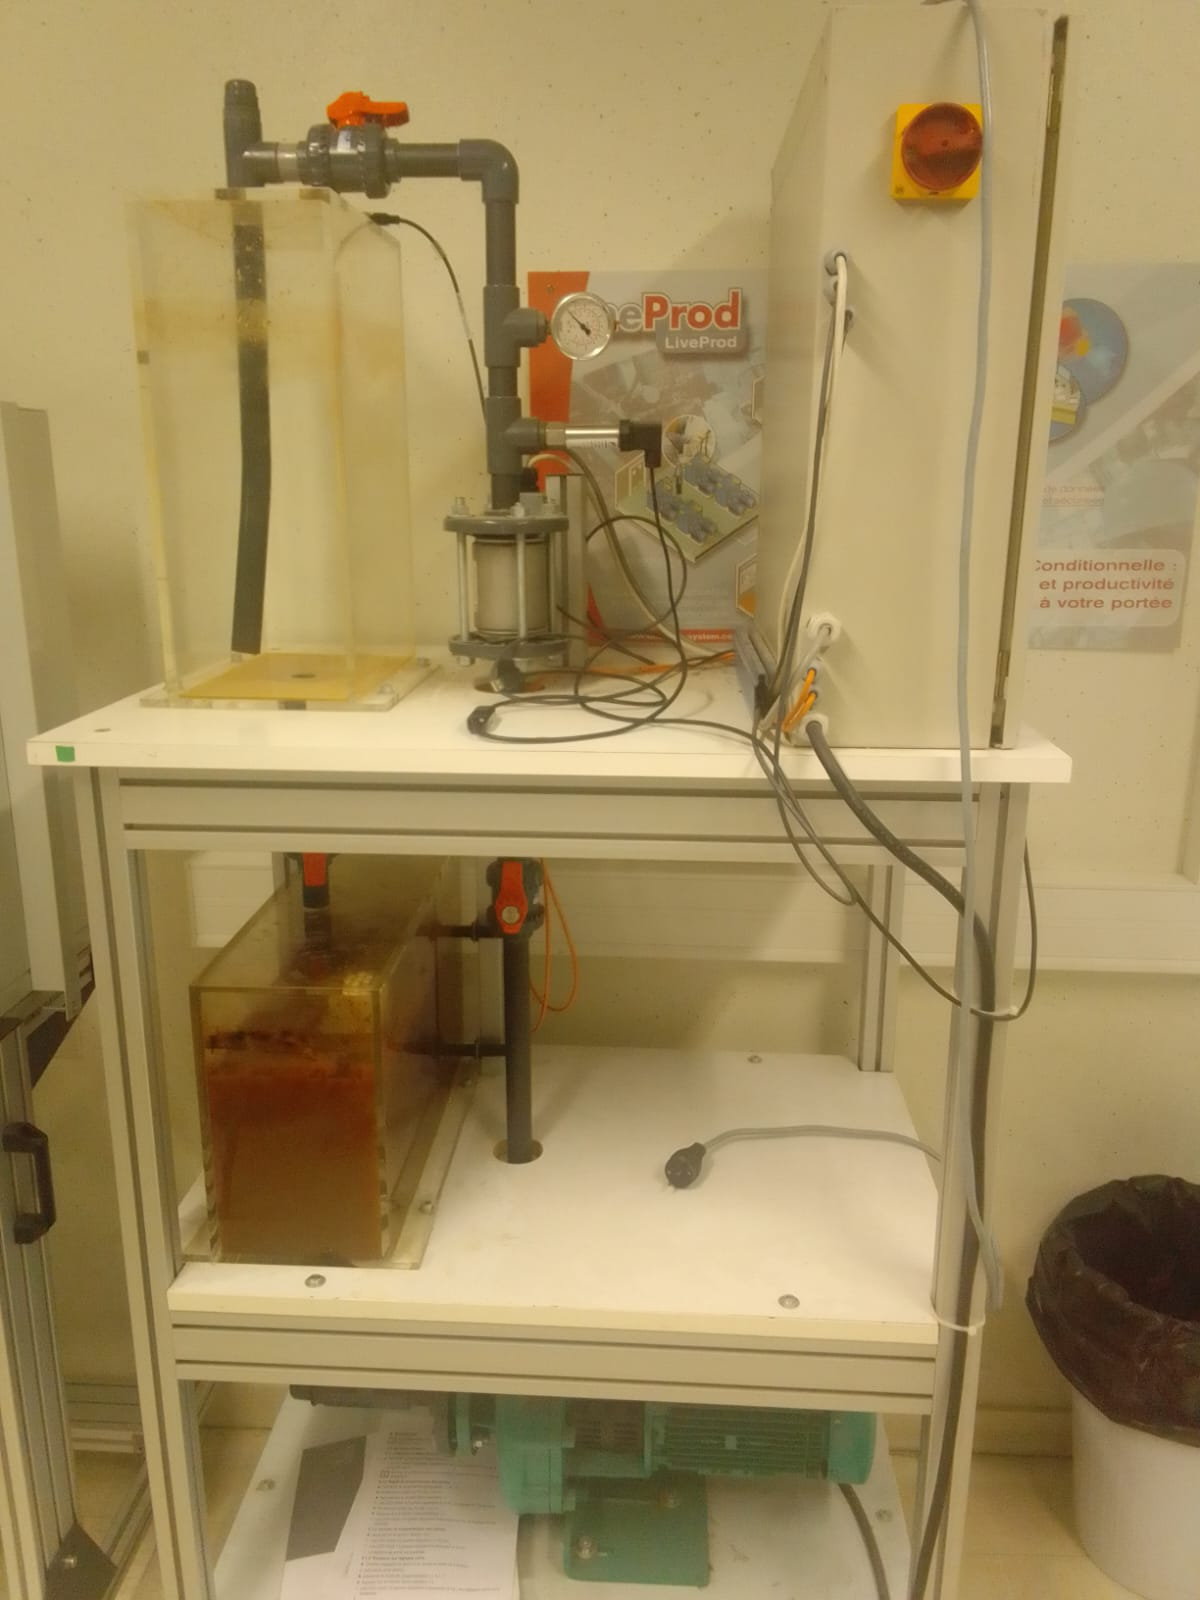
\includegraphics[width=0.48\textwidth]{src/img_chap1/image.png}
    \hfill
    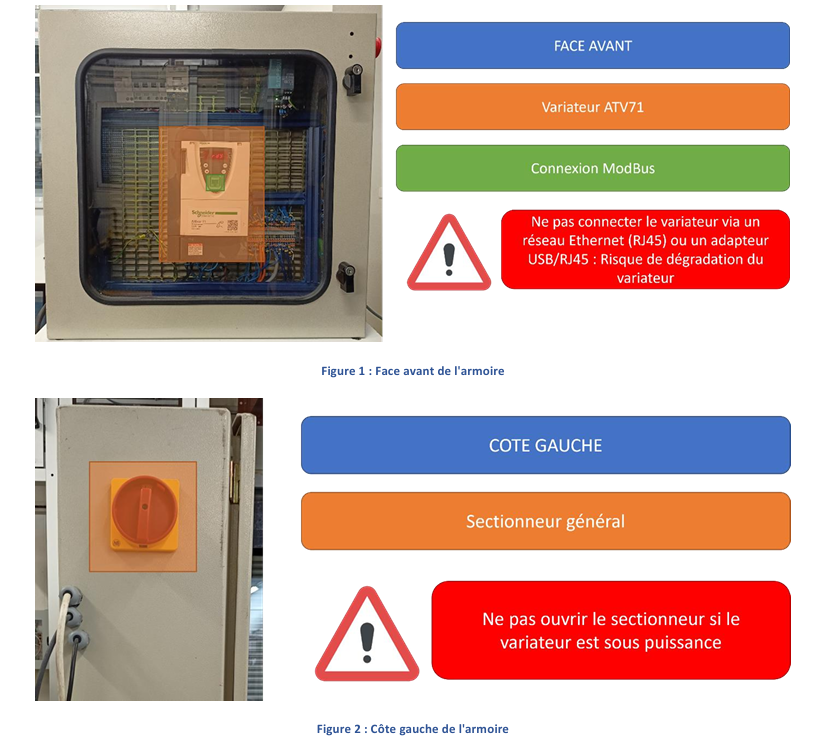
\includegraphics[width=0.48\textwidth]{src/img_chap1/image_2.png}
    \caption{Vue générale du banc d’essai et du circuit hydraulique.}
\end{figure}

\begin{figure}[H]
    \centering
    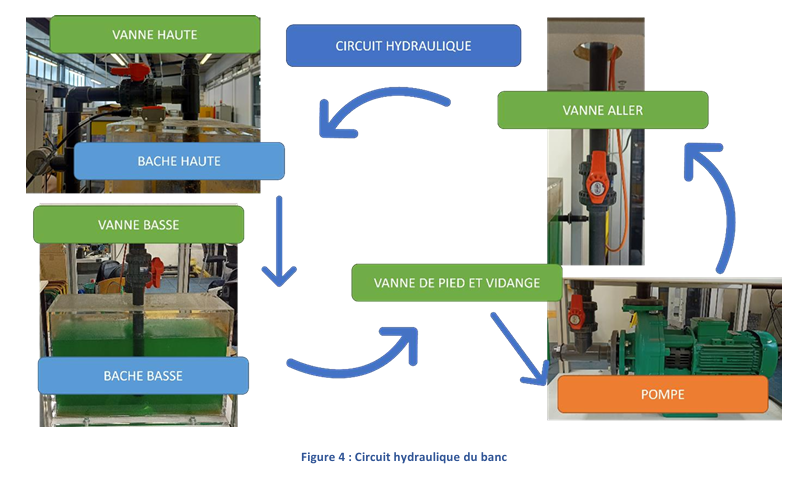
\includegraphics[width=0.75\textwidth]{src/img_chap1/image_3.png}
    \caption{Détail des capteurs et du système de mesure.}
\end{figure}

\section{Identification des capteurs}

\subsection{Capteur BCS00LM : commutateur digital}

\begin{center}
\begin{tikzpicture}
    \node[anchor=south west, inner sep=0] (img1) at (0,0) {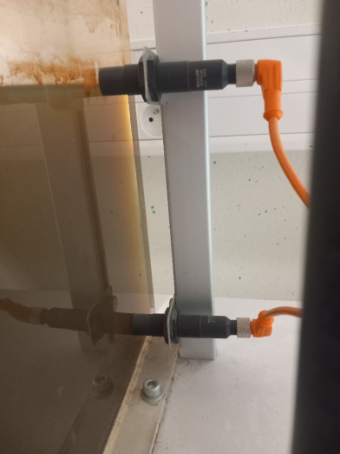
\includegraphics[width=0.5\textwidth]{src/img_chap1/image_BCS00LM.png}};
    \begin{scope}[x={(img1.south east)}, y={(img1.north west)}]
        \draw[blue, line width=3pt, <->, >=latex] (0.6, 0.25) -- (0.6, 0.85);
        \node[draw, fill=white, minimum width=2.5cm, inner sep=2mm] (box1) at (-0.3, 0.55) {\textbf{BCS00LM}};
        \draw[blue, line width=3pt, -latex] (box1.east) -- (0.6, 0.55);
    \end{scope}
\end{tikzpicture}
\end{center}


\subsection{Capteur UGT582 : Détecteur à ultrasons}

\begin{center}
\begin{tikzpicture}
    \node[anchor=south west, inner sep=0] (img2) at (0,0) {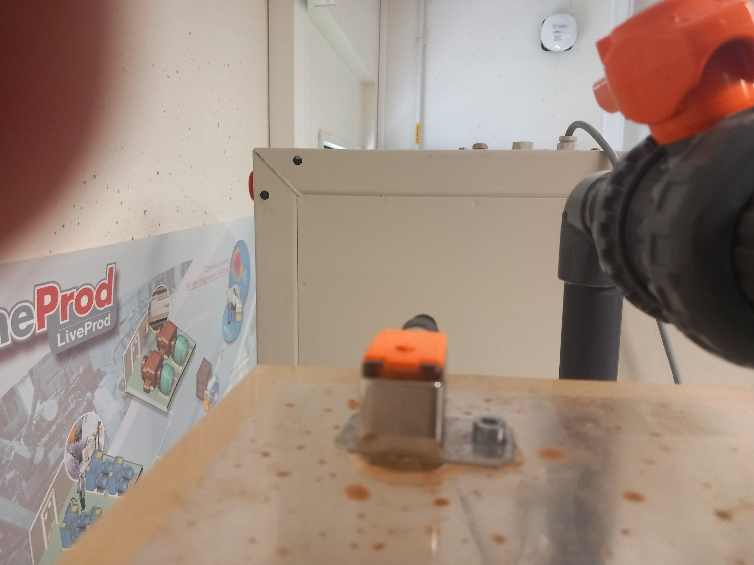
\includegraphics[width=0.5\textwidth]{src/img_chap1/image_UGT582.png}};
    \begin{scope}[x={(img2.south east)}, y={(img2.north west)}]
        \node[draw, fill=white, minimum width=2.5cm, inner sep=2mm] (box2) at (-0.3, 0.25) {\textbf{UGT582}};
        \draw[blue, line width=3pt, -latex] (box2.east) -- (0.5, 0.25);
    \end{scope}
\end{tikzpicture}
\end{center}


\subsection{Capteur GR3000A00 : capteur de pression}

\begin{center}
\begin{tikzpicture}
    \node[anchor=south west, inner sep=0] (img3) at (0,0) {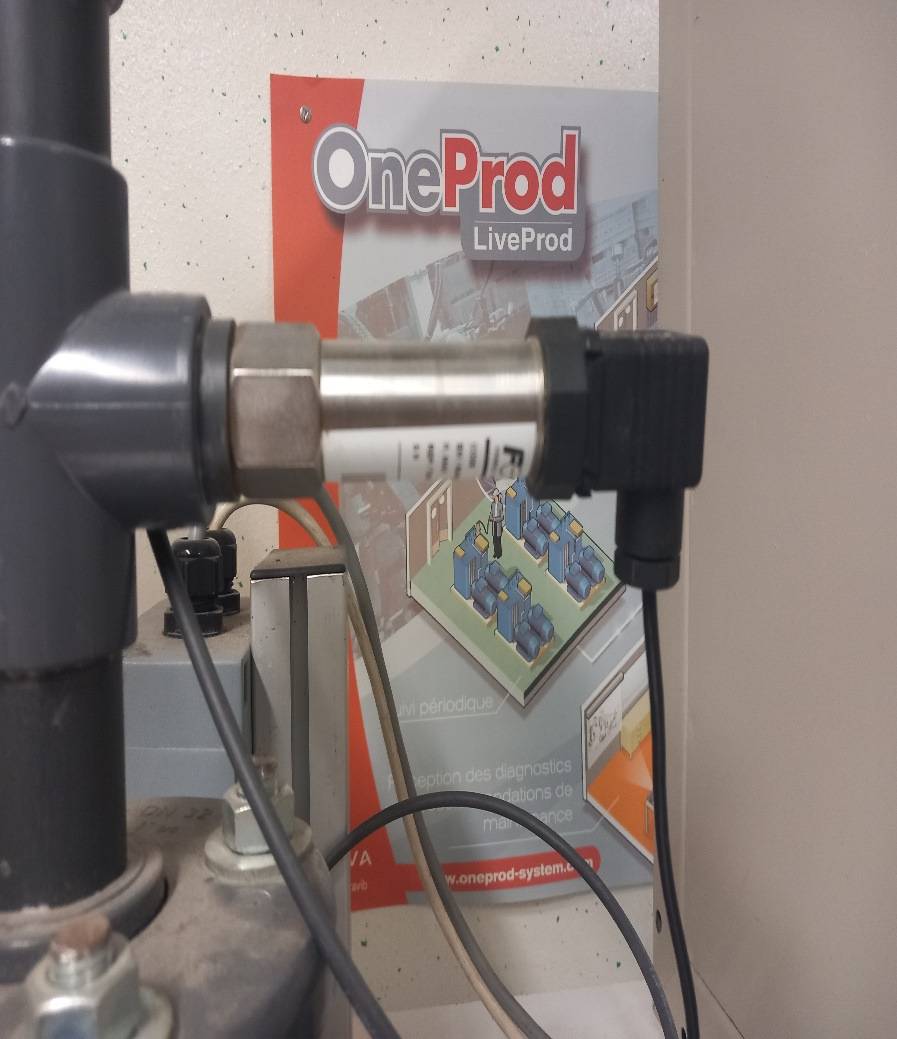
\includegraphics[width=0.5\textwidth]{src/img_chap1/image_GR3000A00.png}};
    \begin{scope}[x={(img3.south east)}, y={(img3.north west)}]
        \draw[blue!80!cyan, line width=4pt, -stealth] (-0.15, 0.35) -- (0.45, 0.35) -- (0.45, 0.50);
        \node[draw, fill=white, minimum width=2.8cm, inner sep=2mm] (box3) at (-0.15, 0.35) {\textbf{GR3000A00}};
    \end{scope}
\end{tikzpicture}
\end{center}


\subsection{Capteur M1000 : le débitmètre électromagnétique}

\begin{center}
\begin{tikzpicture}
    \node[anchor=south west, inner sep=0] (img4) at (0,0) {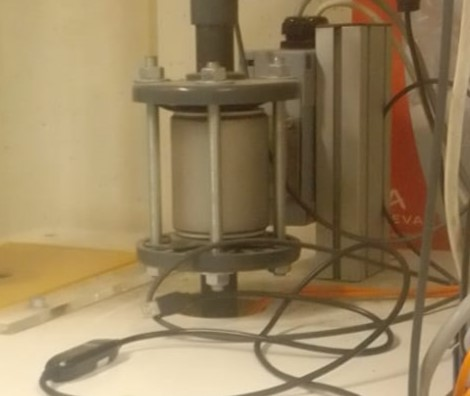
\includegraphics[width=0.5\textwidth]{src/img_chap1/image_M1000.png}};
    \begin{scope}[x={(img4.south east)}, y={(img4.north west)}]
        \draw[blue!80!cyan, line width=4pt, -stealth] (-0.15, 0.45) -- (0.45, 0.45);
        \node[draw, fill=white, minimum width=2.5cm, inner sep=2mm] (box4) at (-0.15, 0.45) {\textbf{M1000}};
    \end{scope}
\end{tikzpicture}
\end{center}


\section{Synthèse des capteurs}

\begin{table}[H]
\centering
\small
\renewcommand{\arraystretch}{1.4}
\begin{tabularx}{\textwidth}{|>{\bfseries}p{2.2cm}|p{3.2cm}|X|c|X|}
\hline
Capteur & Référence & Grandeur mesurée & Plage de mesure & Signal de sortie \\
\hline
M1000 & Débitmètre électromagnétique & Vitesse d'écoulement & 0,03 à 12 m/s & Analogique : 0--4/20 mA ; logique : sorties collecteur ouvert (0--100 Hz / 100--10 000 Hz) ; communication Modbus RTU \\
\hline
UGT582 & UGQ00800E1KG/\allowbreak US & Distance, utilisé pour la mesure du niveau dans la bâche haute & 60 à 800 mm & Signal analogique de 4 à 20 mA \\
\hline
GR3000A00 & GR (transducteur de pression relative) & Pression relative du liquide & -1 à 600 bar & Signal analogique 4 à 20 mA \\
\hline
\end{tabularx}
\caption{Caractéristiques techniques des capteurs du banc d’essai.}
\end{table}

\vspace{5cm}

\section{Récupération des mesures sur le variateur}

Le montage utilisé pour récupérer les mesures des capteurs de pression, de niveau et de débit repose sur des entrées analogiques du variateur ATV71. Les capteurs délivrent un signal électrique représentatif de la grandeur mesurée, qui est ensuite acquis par le variateur afin d’être exploité pour le pilotage et l’analyse du système.

\clearpage

% ==========================================
% PARTIE II
% ==========================================
\part{Démarrage du variateur et acquisition des données}

\section{Communication avec le variateur}

La communication entre l’ordinateur et le variateur se fait par une connexion en série en utilisant le câble « TCSMCNAM3M002P », c’est-à-dire que les données sont transmises bit par bit de manière séquentielle sur un seul canal de communication (contrairement à la liaison parallèle qui envoie plusieurs bits en même temps).

Le câble de communication est branché dans un port série sur l’ordinateur, le port étant l’interface physique sur lequel vient se brancher l’embout du câble. Une fois la connexion enclenchée, le variateur et le PC communiquent en s’envoyant des informations sur leur état.

La vitesse d’envoi de ces bits à travers le canal de communication est exprimée en Bauds. Un bit de parité est parfois rajouté lors de la transmission d’information : celui-ci sert à contrôler l’erreur. Sa valeur dépend des autres bits de façon à ce que la somme des bits à 1 (bit de parité compris) soit toujours paire. Cela permet donc de détecter simplement une possible erreur de la donnée reçue.

D’autres bits peuvent être ajoutés pour fluidifier la communication, notamment l’implémentation de bits d’arrêt qui permet d’indiquer au récepteur que la totalité d’un paquet (un paquet est généralement équivalent à 8 bits) lui a été transmis. De cette façon, le récepteur traite les informations efficacement.

Dans notre cas, la communication entre le variateur et le PC est faite via le protocole de communication MODBUS. Ce dernier est très utilisé pour établir des communications de type maître/client vers esclaves/serveurs (l’appareil principal initie la communication et les appareils secondaires se contentent de répondre). Le protocole MODBUS existe en deux versions :
\begin{itemize}
    \item \textbf{Mode ASCII :} Chaque partie de la trame est transmise sous forme de 2 caractères ASCII (16 bits). Cela a pour avantage d’éviter de générer des erreurs de transmissions.
    \item \textbf{Mode RTU :} Chaque partie de la trame est transmise sous la forme de 2 caractères hexadécimaux de 4 bits (8 bits). Ce qui permet de transmettre les informations plus rapidement.
\end{itemize}

\begin{figure}[H]
    \centering
    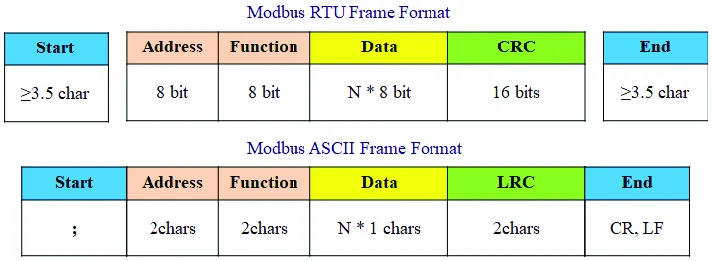
\includegraphics[width=0.75\textwidth]{src/img_chap2/image.png}
    \caption{Structure d'une trame MODBUS.}
\end{figure}

La structure d’une trame MODBUS est la même pour les requêtes (message du maître vers l’esclave) et les réponses (message de l’esclave vers le maître), voir Figure ci-dessus.

\section{Acquisition des données}

Une fois le logiciel SoMove lancé, on configure correctement l’acquisition des données via les annexes disponibles à la fin de l’énoncé de TP, voir ci-dessous.

\begin{figure}[H]
    \centering
    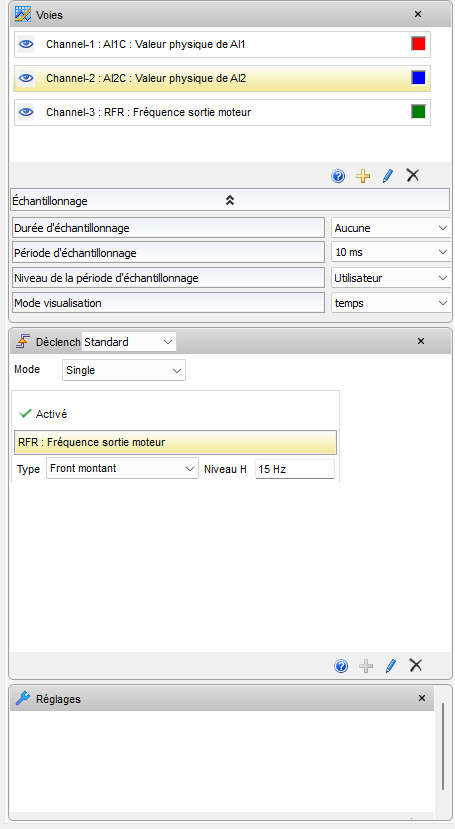
\includegraphics[width=0.75\textwidth]{src/img_chap2/image_1.png}
    \caption{Configuration de l'acquisition sur SoMove.}
\end{figure}

On choisit une période d’échantillonnage de 10 ms, de façon à avoir une courbe relativement lisse. Quant aux voies d’entrées, on souhaite mesurer les signaux : AI1, AI2 et RFR. Après des essais sur la plateforme expérimentale, on en conclut que : 
\begin{itemize}
    \item \textbf{AI1} représente la consigne de notre système, exprimée en Volts.
    \item \textbf{AI2} représente l’évolution du signal de sortie de notre système, qui peut donc représenter l’évolution de la pression, du niveau ou du débit.
    \item \textbf{RFR} représente la fréquence de sortie du moteur, réglable grâce au variateur.
\end{itemize}

À noter que les valeurs de la sortie du système sont exprimées en Ampères (plus précisément en mA). Il est donc impératif, pour obtenir la grandeur physique réelle, de convertir celle-ci en Pascal, mètre cube par seconde ou mètre en fonction du type d’acquisition. On se réfère donc à la documentation technique des différents capteurs.


\subsection{Capteur niveau : détecteur à ultrason UGT582}

D’après la documentation technique, la portée du capteur est comprise entre 60 et 800 mm, tandis que la sortie analogique est comprise dans une plage de 4 à 20 mA. On a donc la formule suivante qui est simplement un produit en croix : 

\begin{equation*}
    \boxed{D = D_{\mathrm{min}} + \frac{I - I_{\mathrm{min}}}{I_{\mathrm{max}} - I_{\mathrm{min}}} \times (D_{\mathrm{max}} - D_{\mathrm{min}})}
\end{equation*}

Avec :
\begin{itemize}
    \item $D$ : niveau de la cuve
    \item $D_{\mathrm{min}}$ et $D_{\mathrm{max}}$ : la portée du capteur (respectivement 60 et 800 mm)
    \item $I$ : courant mesuré par le capteur
    \item $I_{\mathrm{min}}$ et $I_{\mathrm{max}}$ : la plage de courant de la sortie analogique (respectivement 4 et 20 mA)
\end{itemize}

Soit au final :
\begin{center}
    \fbox{$D = 46,25 \times I - 125$}
\end{center}


\subsection{Capteur de pression : transducteur de pression relative -- GR3000A00}

On procède de la même manière que pour le capteur de niveau, le signal de sortie étant lui aussi un courant variant entre 4 et 20 mA. Pour ce qui est de l'étendue de mesure de pression, la documentation indique une plage de -1 à 600 bars sur 31 échelles. Le modèle pouvant être configuré sur plusieurs plages (exemple : 0 à 10 bars, ...). 

Ainsi, on obtient une formule similaire à celle trouvée précédemment :
\begin{equation*}
    \boxed{P = P_{\mathrm{min}} + \frac{I - I_{\mathrm{min}}}{I_{\mathrm{max}} - I_{\mathrm{min}}} \times (P_{\mathrm{max}} - P_{\mathrm{min}})}
\end{equation*}


\subsection{Capteur de débit : M1000}

Pour obtenir le débit d'eau entrant dans la cuve, il est nécessaire de faire davantage de calculs. D'après la documentation, le débit est exprimé en mètre par seconde et l'échelle de mesure est comprise entre 0,03 et 12 m/s. C'est en fait la vitesse d'écoulement de l'eau et non le débit. C'est pourquoi, pour bien obtenir le débit, il faut multiplier la vitesse de l'eau entrant dans la cuve par la section du tuyau, soit :

\begin{equation*}
    \boxed{Q = V \times S = V \times \frac{\pi D^2}{4}}
\end{equation*}

Avec :
\begin{itemize}
    \item $V$ : Vitesse d'écoulement de l'eau (m/s)
    \item $S$ : Section intérieure du tuyau (m$^2$)
    \item $Q$ : Débit (m$^3$/s)
    \item $D$ : Diamètre du tuyau (m)
\end{itemize}

On obtient donc :
\begin{equation*}
    \boxed{V = V_{\mathrm{min}} + \frac{I - 4}{20 - 4}(V_{\mathrm{max}} - V_{\mathrm{min}})}
\end{equation*}

Soit finalement :
\begin{equation*}
    \boxed{Q(I) = \frac{\pi D^2}{4} \left[ V_{\mathrm{min}} + \frac{I - 4}{16}(V_{\mathrm{max}} - V_{\mathrm{min}}) \right]}
\end{equation*}

En remplaçant par les valeurs connues :
\begin{equation*}
    \boxed{Q(I) = \frac{\pi D^2}{4} \big[ 0,03 + 0,748125(I - 4) \big]}
\end{equation*}

Ainsi, les différentes formules pour le débit, la pression et le niveau pourraient permettre, dans le cas d’un asservissement, de traiter les données physiques de l’évolution du système.

\clearpage

% ==========================================
% PARTIE III
% ==========================================
\part{Analyse des résultats expérimentaux}

\section{Caractérisation des réponses indicielles (échelon de vitesse)}

Afin d'étudier la dynamique du système hydraulique, nous avons appliqué des échelons de vitesse au moteur de la pompe (passage brusque d'une fréquence nulle à une fréquence de consigne, par exemple 15, 20 ou 30 Hz) et enregistré la réponse des différents capteurs via le logiciel SoMove.

Les relevés ont été effectués en modifiant systématiquement les conditions initiales du circuit hydraulique : tuyauterie initialement vide ou tuyauterie déjà pleine. 

\subsection{Évolution du débit}

Les figures ci-dessous illustrent la réponse en débit pour des échelons de vitesse de 15 Hz et 20 Hz, selon que le tuyau est initialement plein ou vide.

\begin{figure}[H]
    \centering
    \begin{minipage}{0.48\textwidth}
        \centering
        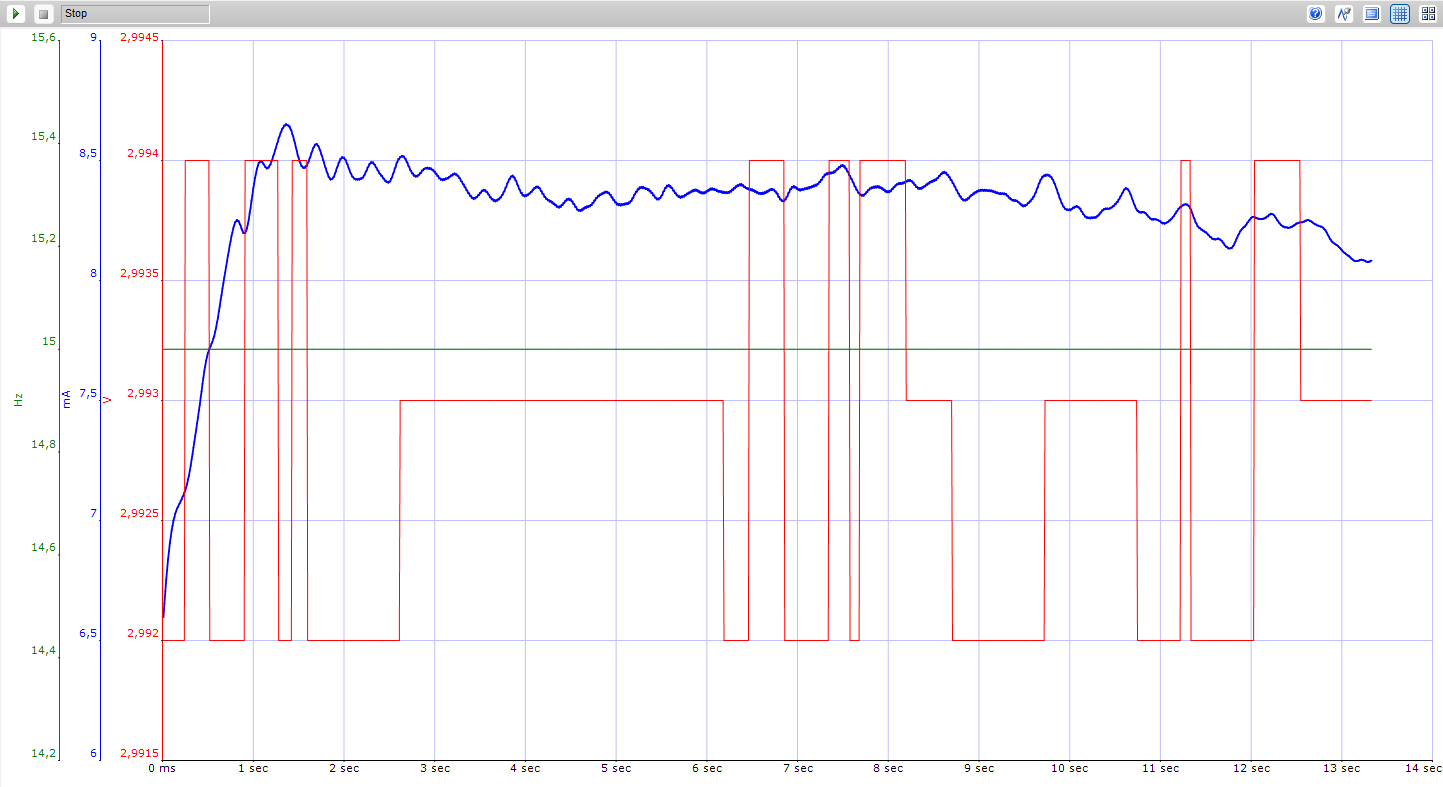
\includegraphics[width=\textwidth]{src/img_chap3/Test_debit_15Hz_plein.png}
        \caption{Débit à 15 Hz (Tuyau plein)}
    \end{minipage}
    \hfill
    \begin{minipage}{0.48\textwidth}
        \centering
        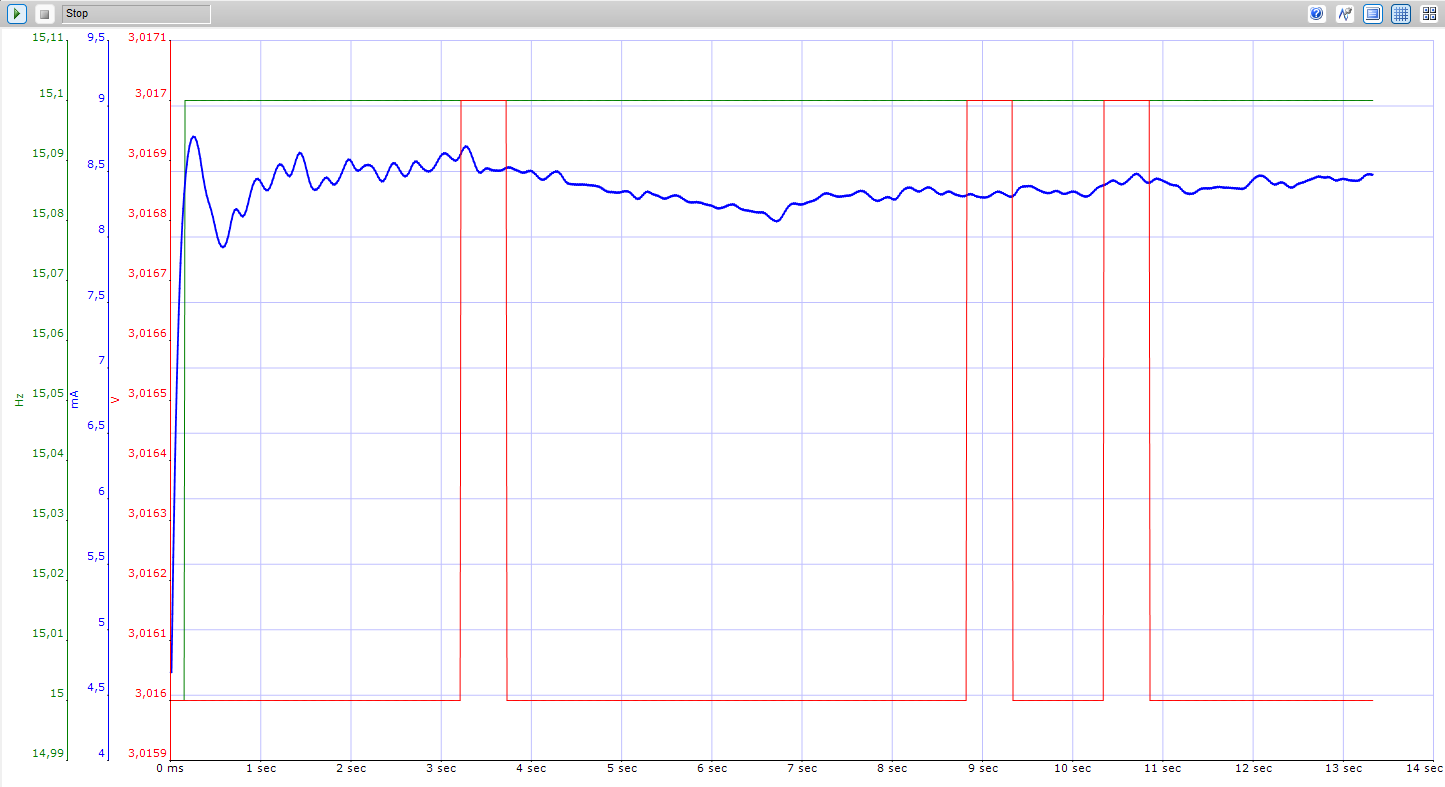
\includegraphics[width=\textwidth]{src/img_chap3/Test_debit_15Hz_vide.png}
        \caption{Débit à 15 Hz (Tuyau vide)}
    \end{minipage}
\end{figure}

\textbf{Observations à 15 Hz :} 
Lorsque le tuyau est plein, le débit augmente quasi-instantanément pour atteindre son régime permanent, avec une dynamique qui s'apparente à un système du premier ordre rapide.
En revanche, lorsque le tuyau est vide, on observe un \textbf{retard pur} (temps mort) très significatif de plusieurs secondes. Ce temps correspond au délai physique nécessaire pour que l'eau remplisse la tuyauterie et atteigne le capteur. On remarque également une oscillation transitoire importante lors de l'arrivée brutale de l'eau dans le débitmètre.

\begin{figure}[H]
    \centering
    \begin{minipage}{0.48\textwidth}
        \centering
        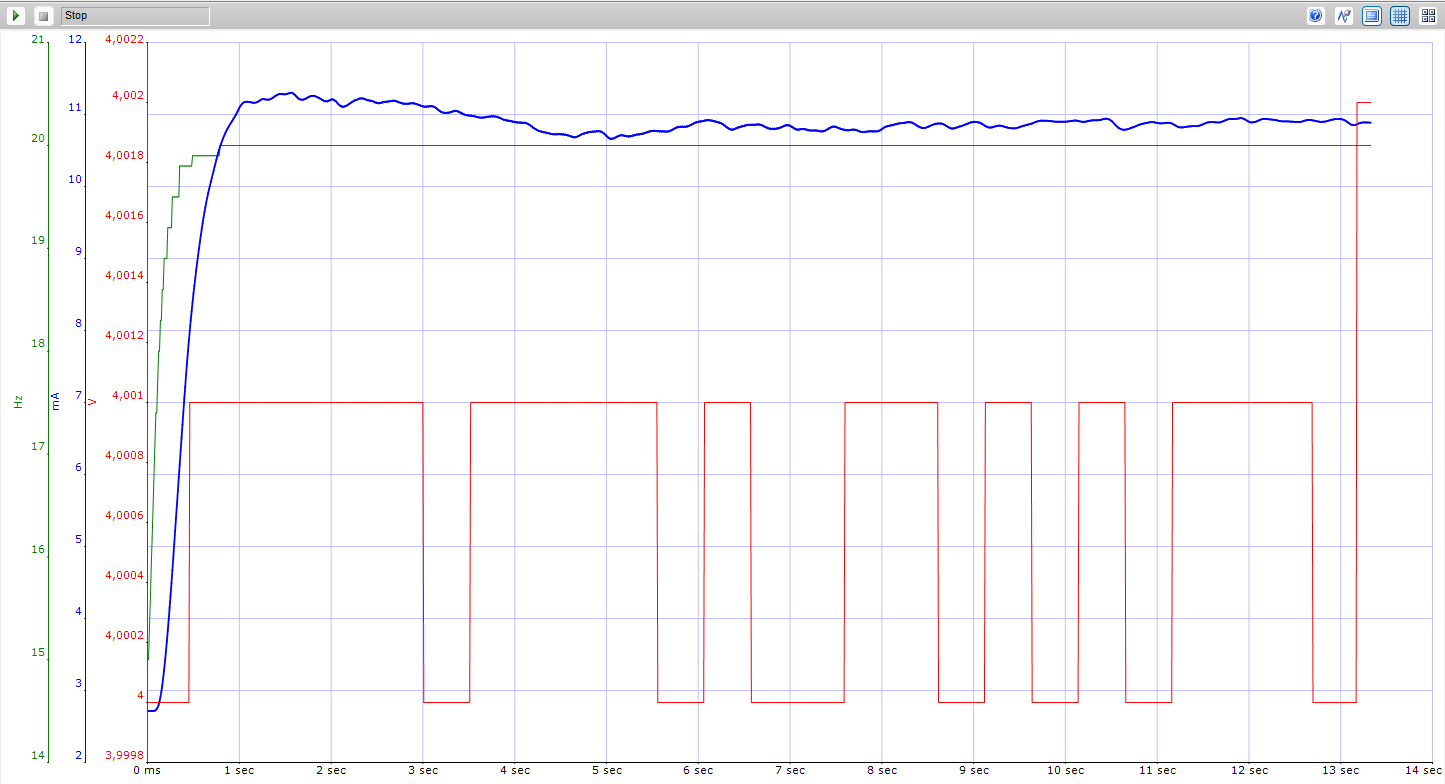
\includegraphics[width=\textwidth]{src/img_chap3/Test_debit_20Hz_plein.png}
        \caption{Débit à 20 Hz (Tuyau plein)}
    \end{minipage}
    \hfill
    \begin{minipage}{0.48\textwidth}
        \centering
        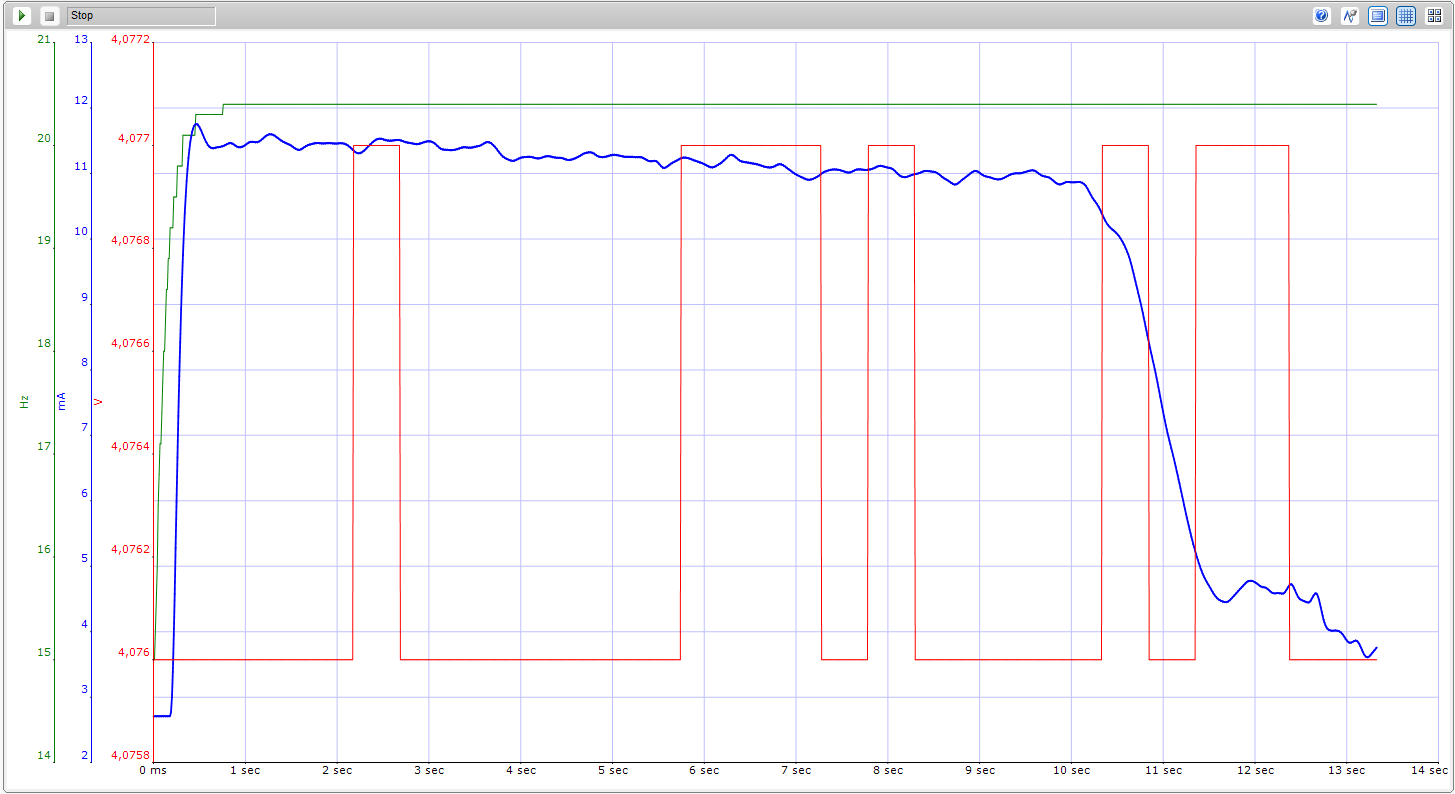
\includegraphics[width=\textwidth]{src/img_chap3/Test_debit_20Hz_vide.png}
        \caption{Débit à 20 Hz (Tuyau vide)}
    \end{minipage}
\end{figure}

\textbf{Observations à 20 Hz :} 
L'augmentation de l'échelon (passage à 20 Hz) permet d'atteindre un débit final plus élevé et réduit légèrement ce temps mort, la pompe débitant davantage et remplissant la tuyauterie plus rapidement. La dynamique globale d'établissement du régime permanent reste similaire.

\subsection{Évolution de la pression}

Une démarche similaire a été réalisée pour la mesure de pression avec des échelons plus élevés (30 Hz et 50 Hz), car pour voir une évolution plus claire de la pression.

\begin{figure}[H]
    \centering
    \begin{minipage}{0.48\textwidth}
        \centering
        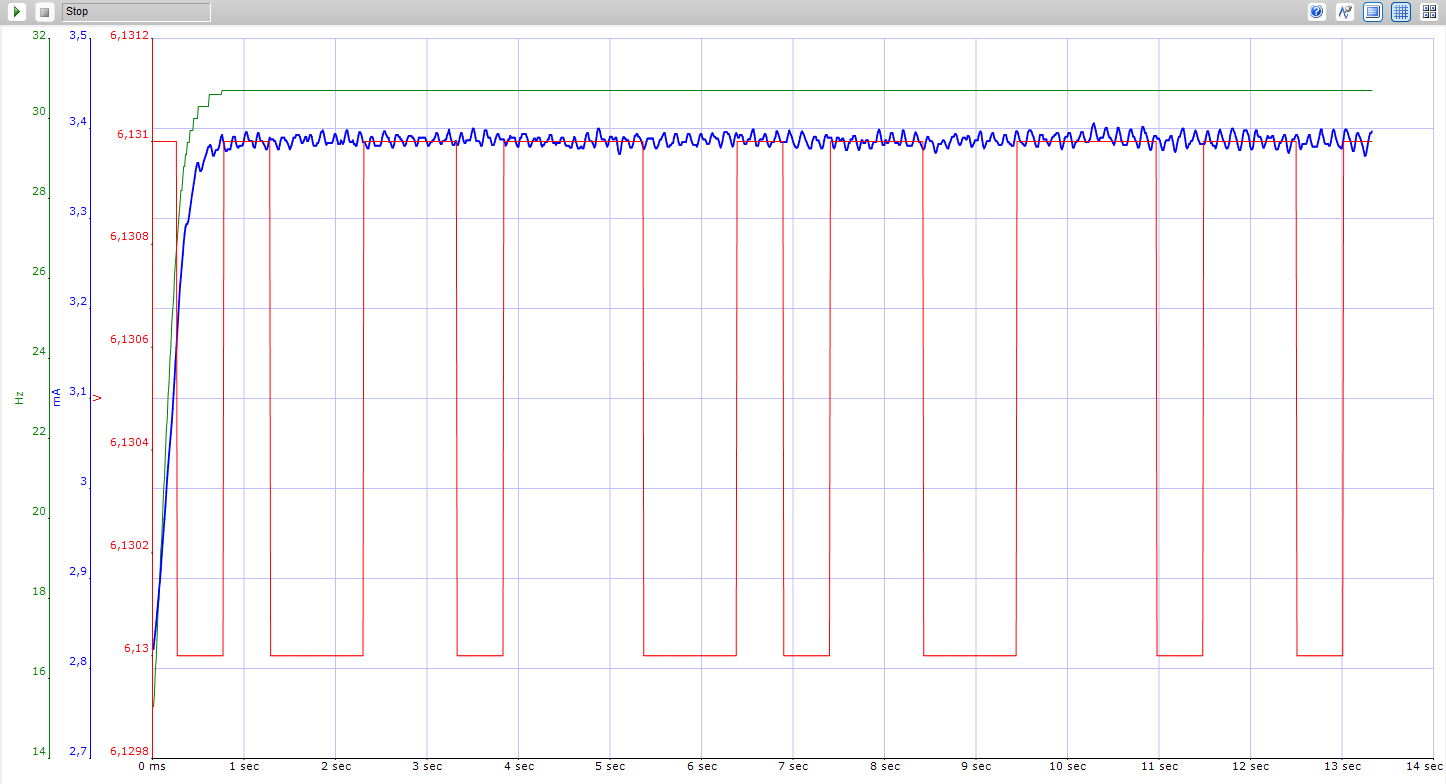
\includegraphics[width=\textwidth]{src/img_chap3/Test_pression_tuyau_plein_30Hz.png}
        \caption{Pression à 30 Hz (Tuyau plein)}
    \end{minipage}
    \hfill
    \begin{minipage}{0.48\textwidth}
        \centering
        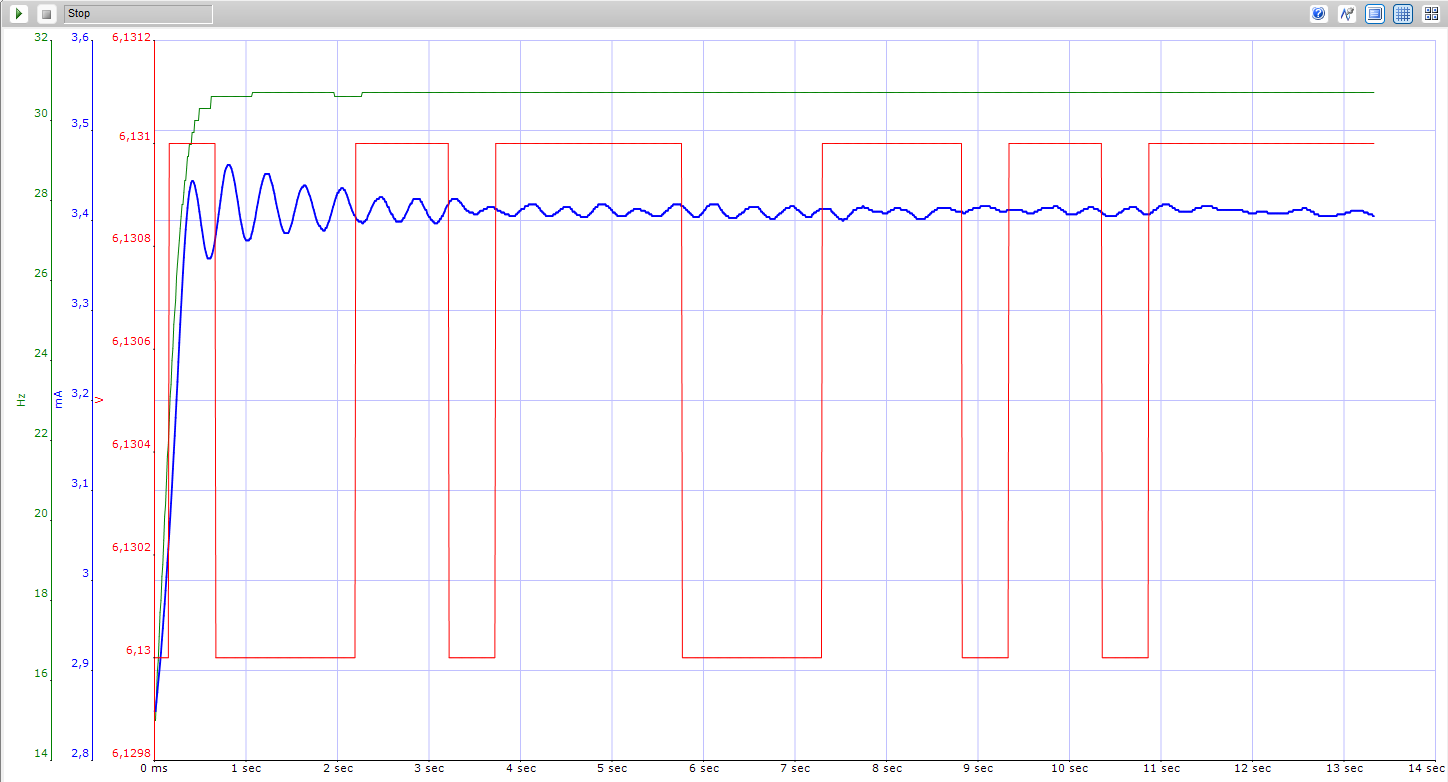
\includegraphics[width=\textwidth]{src/img_chap3/Test_pression_tuyau_vide_30Hz.png}
        \caption{Pression à 30 Hz (Tuyau vide)}
    \end{minipage}
\end{figure}

\textbf{Observations à 30 Hz :} 
La dynamique de la pression est extrêmement rapide. À tuyau plein, la montée en pression est quasi-instantanée. On note une forte composante bruitée (ondulations) en régime permanent, qui est due aux turbulences de l'eau et au hachage mécanique des pales de la pompe. 
À tuyau vide, le temps mort est présent, suivi d'une importante oscillation transitoire ("coup de bélier") lorsque la colonne d'eau vient frapper les parois et le capteur, avant que le signal ne se stabilise.

\begin{figure}[H]
    \centering
    \begin{minipage}{0.48\textwidth}
        \centering
        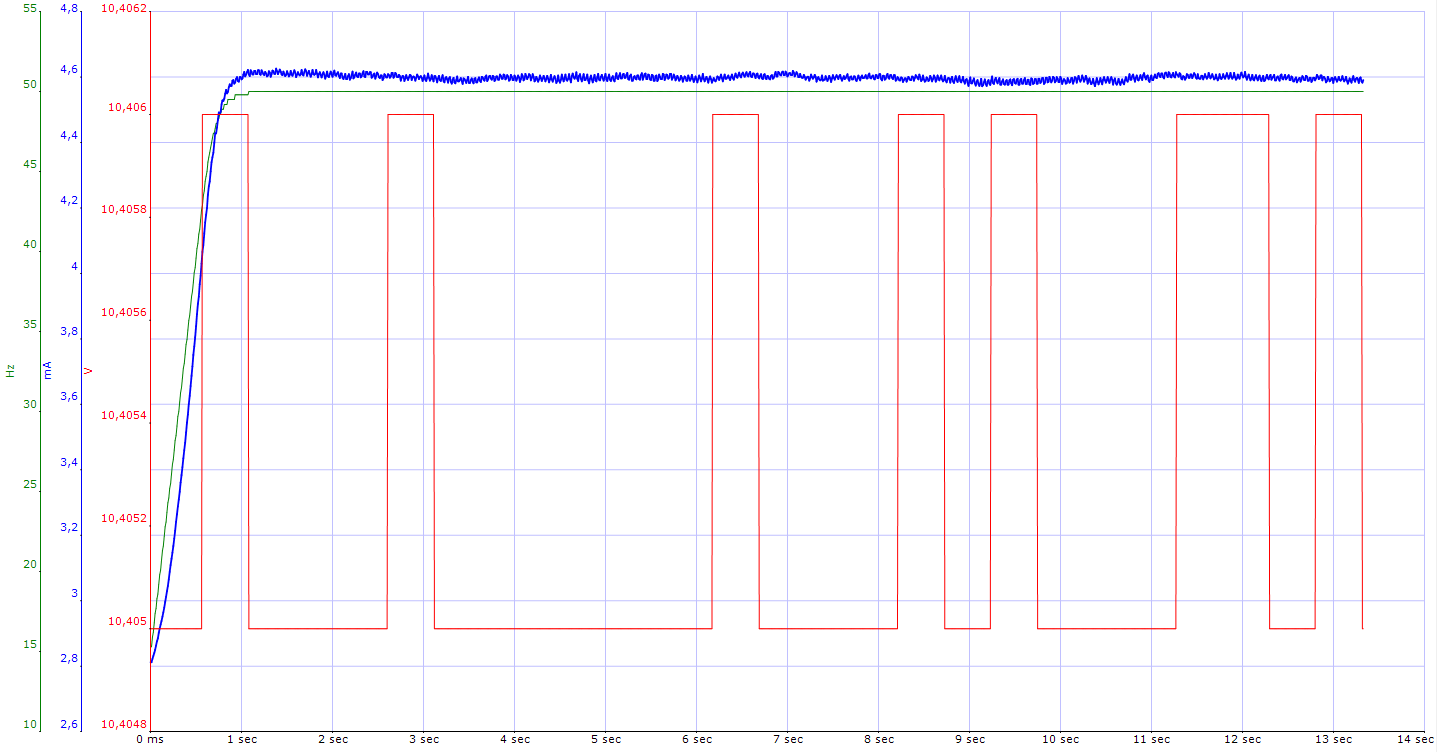
\includegraphics[width=\textwidth]{src/img_chap3/Test_pression_tuyau_rempli_50Hz.png}
        \caption{Pression à 50 Hz (Tuyau plein)}
    \end{minipage}
    \hfill
    \begin{minipage}{0.48\textwidth}
        \centering
        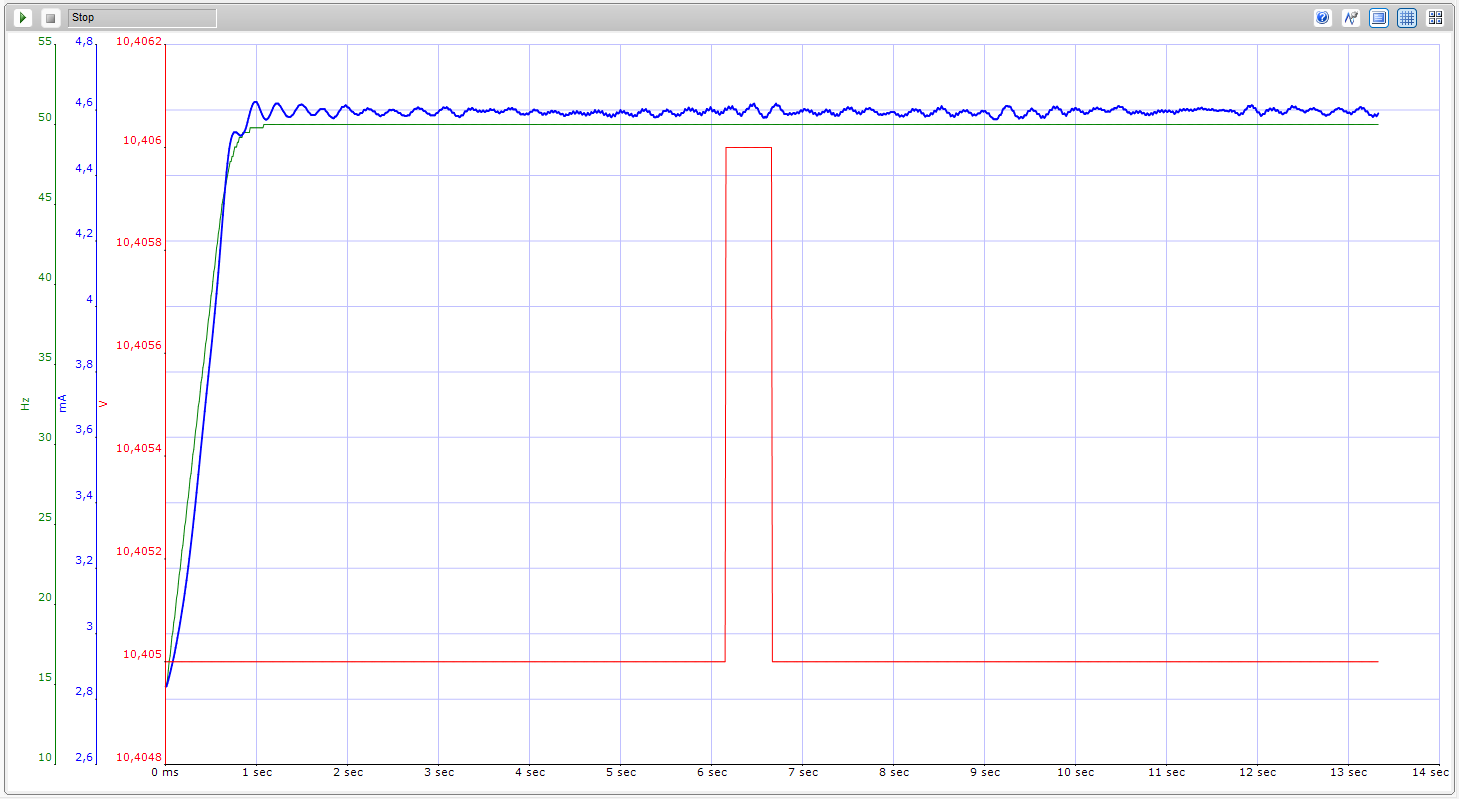
\includegraphics[width=\textwidth]{src/img_chap3/Test_pression_tuyau_vide_50Hz.png}
        \caption{Pression à 50 Hz (Tuyau vide)}
    \end{minipage}
\end{figure}

\textbf{Observations à 50 Hz :} 
L'augmentation de la consigne de vitesse permet logiquement d'atteindre un niveau de pression statique plus élevé. De la même manière que pour le débit, le temps mort initial observé à tuyau vide est légèrement réduit, la pompe remplissant le circuit plus rapidement. Le dépassement transitoire et le bruit de mesure restent des caractéristiques dominantes de ce signal.
\subsection{Évolution du niveau}

D'un point de vue théorique, contrairement au débit et à la pression qui se stabilisent rapidement à une valeur constante (régime permanent) pour une vitesse donnée, le niveau dans la bâche haute présente un comportement différent. Si la vanne de fuite est fermée, la hauteur d'eau ne cesse de croître selon une pente proportionnelle au débit d'entrée. Si la vanne est ouverte, le système s'équilibre lorsque le débit de fuite compense exactement le débit entrant.

Néanmoins, lors de nos essais pratiques, nous avons été confrontés à un dysfonctionnement technique concernant le capteur de niveau à ultrasons (UGT582). En effet, celui-ci présentait une anomalie de détection : la mesure ne s'activait qu'à partir d'un certain seuil de remplissage, lorsque le niveau d'eau était déjà particulièrement haut dans la bâche. 

Afin de pallier ce problème, plusieurs opérations de dépannage ont été entreprises, notamment la vérification et le repositionnement physique du capteur (pour éviter d'éventuels échos parasites sur les parois) ainsi qu'une tentative de reparamétrage de ses seuils de fonctionnement. Malgré ces interventions, la défaillance a persisté. Cette contrainte matérielle nous a donc empêchés d'acquérir un relevé expérimental complet et exploitable de la dynamique de remplissage de la cuve depuis son état vide.


\clearpage

% ==========================================
% CONCLUSION
% ==========================================
\part{Conclusion}

Ce premier travail pratique a constitué une étape préparatoire fondamentale dans l'appréhension du banc de régulation niveau-débit-pression. Avant d'envisager la synthèse d'un quelconque correcteur, il était indispensable de maîtriser la chaîne d'acquisition et de comprendre intimement la physique du système.

Dans un premier temps, l'étude s'est concentrée sur l'instrumentation, nous permettant de faire le lien direct entre les grandeurs physiques réelles (fluides) et les signaux électriques (4-20 mA) traités par le variateur ATV71 via le protocole Modbus. L'établissement rigoureux des lois de conversion mathématiques a garanti une interprétation correcte des données brutes issues du logiciel SoMove.

L'analyse expérimentale des réponses indicielles a ensuite mis en exergue la complexité dynamique de ce circuit hydraulique. Nous avons pu constater que le système est fortement non-linéaire et conditionné par son état initial. La présence de retards purs importants (temps morts liés au remplissage des tuyauteries à vide), couplée à des phénomènes de turbulences et de bruits de mesure (particulièrement visibles sur les relevés de pression), constitue un défi majeur. À cela s'est ajoutée la confrontation à une défaillance matérielle réelle avec le capteur de niveau à ultrasons, soulignant l'importance de l'esprit critique et du diagnostic en ingénierie d'essais.

En perspective, ces observations démontrent qu'une simple régulation PID standard risque de se révéler inadaptée ou très instable si elle n'est pas précautionneusement paramétrée. La suite logique de cette étude nécessitera la mise en place d'un filtrage numérique pour lisser les signaux (atténuation du bruit), ainsi que l'élaboration de stratégies de commande robustes, spécifiquement conçues pour anticiper les retards purs et s'adapter aux différentes dynamiques de la pression, du débit et du niveau.

\clearpage
% ==============================================================================
% BIBLIOGRAPHIE ET RÉFÉRENCES
% ==============================================================================
% ==========================================
% BIBLIOGRAPHIE
% ==========================================
\addcontentsline{toc}{section}{Références}
\begin{thebibliography}{9}

\bibitem{Détecteur à ultrasons - UGT582 - ifm}
\textbf{Détecteur à ultrasons - UGT582}, \textit{ifm electronic}.\\
\url{https://www.ifm.com/fr/fr/product/UGT582}\\
\small{Documentation technique officielle du constructeur. Cette source a permis d'extraire la portée du capteur (60 à 800 mm) ainsi que les caractéristiques de son signal de sortie analogique (4-20 mA) afin d'établir, par le calcul, la loi de conversion liant le courant mesuré au niveau d'eau réel dans la cuve.}

\vspace{0.5cm}

\bibitem{Transducteur de pression relative - GR | Fuji Electric}
\textbf{Transducteur de pression relative - Série GR}, \textit{Fuji Electric}.\\
\url{https://www.fujielectric.fr/produit/mesure-de-pression/transducteur-de-pression-relative-gr/}\\
\small{Fiche technique du capteur de pression. Elle détaille l'étendue de mesure couverte (jusqu'à 31 échelles de -1 à 600 bars) et le fonctionnement du signal 4-20 mA. Ces données constructeurs justifient la modélisation de la relation linéaire entre le signal acquis par le variateur et la pression physique du fluide.}

\vspace{0.5cm}

\bibitem{Débitmètre électromagnétique M1000}
\textbf{Débitmètre électromagnétique M1000}, \textit{Fuji Electric}.\\
\url{https://www.fujielectric.fr/technologies/debitmetre-electromagnetique-economique-m1000/}\\
\small{Documentation du débitmètre, essentielle pour comprendre et justifier l'équation de calcul du débit. Elle précise notamment que l'appareil mesure directement une vitesse d'écoulement (de 0,03 à 12 m/s) et non un débit volumique, expliquant ainsi la nécessité d'intégrer la section géométrique du tuyau dans nos formules.}

\end{thebibliography}

% ==============================================================================
% TABLE DES ILLUSTRATIONS
% ==============================================================================

\listoffigures
\cleardoublepage

\end{document}